% Architektur und Datenfluss des Benchmark-Frameworks (Abschnitt 3.2)
% Eigenstaendig kompilierbar (pdflatex architektur.tex -> architektur.pdf),
% in der Arbeit dann per 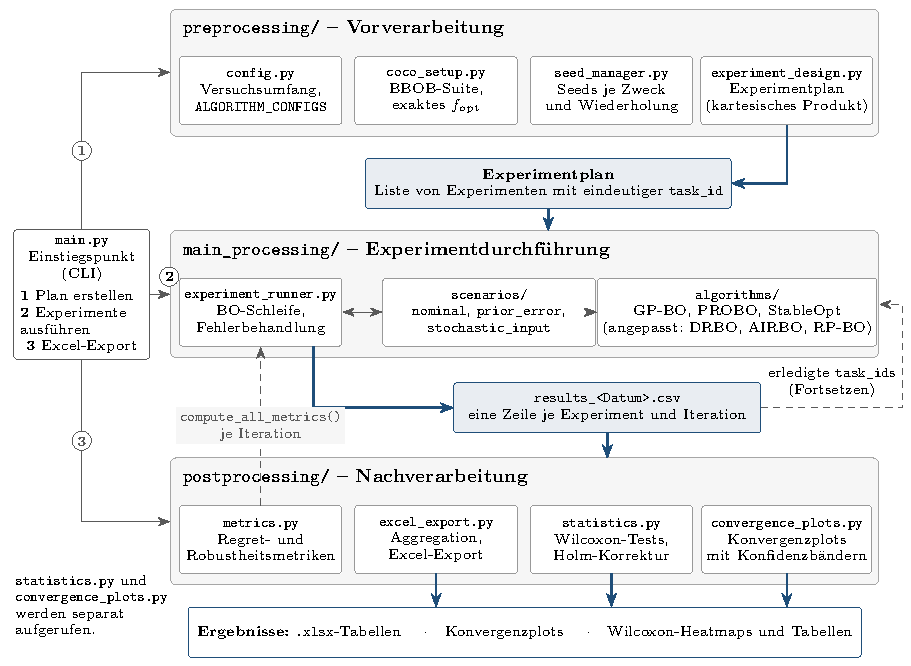
\includegraphics{architektur.pdf} einbinden.
\documentclass[tikz,border=4pt]{standalone}
\usepackage[utf8]{inputenc}
\usepackage[T1]{fontenc}
\usepackage[ngerman]{babel}
\usepackage{lmodern}
\usetikzlibrary{arrows.meta,positioning,shapes.geometric,calc}

\definecolor{akzent}{RGB}{31,78,121}

\begin{document}
\begin{tikzpicture}[
    >={Stealth[length=2.2mm]},
    font=\small,
    layer/.style={draw=gray!70, rounded corners=3pt, fill=gray!7},
    layertitle/.style={anchor=north west, font=\small\bfseries, inner sep=0pt},
    mod/.style={draw=gray!80, fill=white, rounded corners=1.5pt, align=center,
                minimum height=1.15cm, inner sep=2pt, font=\scriptsize},
    data/.style={draw=akzent, fill=akzent!10, rounded corners=1.5pt, align=center,
                 minimum height=0.85cm, inner sep=4pt, font=\scriptsize},
    flow/.style={->, thick, akzent},
    ctrl/.style={->, gray!70!black},
    aux/.style={->, dashed, gray!70!black},
    nr/.style={circle, draw=gray!70!black, fill=white, inner sep=1pt,
                 font=\scriptsize\bfseries},
    lbl/.style={font=\scriptsize, fill=white, inner sep=1.5pt},
]

% Dateinamen in Schreibmaschinenschrift
\newcommand{\f}[1]{{\ttfamily\bfseries #1}}

% ------------------------------------------------------------------
% Schicht 1: preprocessing
% ------------------------------------------------------------------
\draw[layer] (2.6,0) rectangle (14.6,-2.15);
\node[layertitle] at (2.8,-0.18) {\f{preprocessing/} -- Vorverarbeitung};

\node[mod, minimum width=2.75cm] (config) at (4.13,-1.38)
    {\f{config.py}\\Versuchsumfang,\\\texttt{ALGORITHM\_CONFIGS}};
\node[mod, minimum width=2.75cm] (coco) at (7.10,-1.38)
    {\f{coco\_setup.py}\\BBOB-Suite,\\exaktes $f_{\mathrm{opt}}$};
\node[mod, minimum width=2.75cm] (seeds) at (10.07,-1.38)
    {\f{seed\_manager.py}\\Seeds je Zweck\\und Wiederholung};
\node[mod, minimum width=2.75cm] (design) at (13.04,-1.38)
    {\f{experiment\_design.py}\\Experimentplan\\(kartesisches Produkt)};

% Datenobjekt: Experimentplan
\node[data, minimum width=5.2cm] (plan) at (9.0,-2.95)
    {\textbf{Experimentplan}\\Liste von Experimenten mit eindeutiger \texttt{task\_id}};

% ------------------------------------------------------------------
% Schicht 2: main_processing
% ------------------------------------------------------------------
\draw[layer] (2.6,-3.75) rectangle (14.6,-5.9);
\node[layertitle] at (2.8,-3.93) {\f{main\_processing/} -- Experimentdurchführung};

\node[mod, minimum width=2.75cm] (runner) at (4.13,-5.13)
    {\f{experiment\_runner.py}\\BO-Schleife,\\Fehlerbehandlung};
\node[mod, minimum width=3.6cm] (scen) at (8.0,-5.13)
    {\f{scenarios/}\\\texttt{nominal}, \texttt{prior\_error},\\\texttt{stochastic\_input}};
\node[mod, minimum width=4.3cm] (algo) at (12.2,-5.13)
    {\f{algorithms/}\\GP-BO, PROBO, StableOpt\\(angepasst: DRBO, AIRBO, RP-BO)};

\draw[<->, gray!70!black] (runner) -- (scen);
\draw[<->, gray!70!black] (scen) -- (algo);

% Datenobjekt: Ergebnis-CSV
\node[data, minimum width=5.2cm] (csv) at (10.0,-6.75)
    {\texttt{results\_<Datum>.csv}\\eine Zeile je Experiment und Iteration};

% ------------------------------------------------------------------
% Schicht 3: postprocessing
% ------------------------------------------------------------------
\draw[layer] (2.6,-7.6) rectangle (14.6,-9.75);
\node[layertitle] at (2.8,-7.78) {\f{postprocessing/} -- Nachverarbeitung};

\node[mod, minimum width=2.75cm] (metrics) at (4.13,-8.98)
    {\f{metrics.py}\\Regret- und\\Robustheitsmetriken};
\node[mod, minimum width=2.75cm] (excel) at (7.10,-8.98)
    {\f{excel\_export.py}\\Aggregation,\\Excel-Export};
\node[mod, minimum width=2.75cm] (stats) at (10.07,-8.98)
    {\f{statistics.py}\\Wilcoxon-Tests,\\Holm-Korrektur};
\node[mod, minimum width=2.75cm] (plots) at (13.04,-8.98)
    {\f{convergence\_plots.py}\\Konvergenzplots\\mit Konfidenzbändern};

% Ausgaben
\node[data, minimum width=11.4cm, fill=white] (out) at (8.6,-10.55)
    {\textbf{Ergebnisse:} \texttt{.xlsx}-Tabellen \quad$\cdot$\quad Konvergenzplots
     \quad$\cdot$\quad Wilcoxon-Heatmaps und Tabellen};

% ------------------------------------------------------------------
% Datenfluss (blau)
% ------------------------------------------------------------------
\draw[flow] (design.south) |- (plan.east);
\draw[flow] (plan.south) -- (plan.south |- 0,-3.75);
\draw[flow] (runner.south) ++(0.9,0) |- (csv.west);
\draw[flow] (csv.south) -- (csv.south |- 0,-7.6);
\draw[flow] (excel.south) -- (excel.south |- out.north);
\draw[flow] (stats.south) -- (stats.south |- out.north);
\draw[flow] (plots.south) -- (plots.south |- out.north);

% ------------------------------------------------------------------
% Hilfsbeziehungen (gestrichelt)
% ------------------------------------------------------------------
% Runner ruft je Iteration die Metrikberechnung auf
\draw[aux] (metrics.north) -- (runner.south)
    node[midway, lbl, fill=gray!7, align=center]
    {\texttt{compute\_all\_metrics()}\\je Iteration};
% Fortsetzen nach Abbruch: erledigte task_ids aus der CSV lesen
\draw[aux] (csv.east) -- (15.0,-6.75) |- (14.6,-5.0);
\node[font=\scriptsize, align=center] at (13.8,-6.32)
    {erledigte \texttt{task\_id}s\\(Fortsetzen)};

% ------------------------------------------------------------------
% Steuerung durch main.py
% ------------------------------------------------------------------
\node[draw=gray!70!black, fill=white, rounded corners=2pt, align=center,
      text width=2.1cm, inner sep=3pt, font=\scriptsize] (main) at (1.1,-4.83)
    {\centering\f{main.py}\\Einstiegspunkt (CLI)\par\smallskip
     \raggedright\textbf{1} Plan erstellen\\\textbf{2} Experimente ausführen\\\textbf{3} Excel-Export};

\draw[ctrl] (main.north) |- (2.6,-1.07)
    node[pos=0.25, nr] {1};
\draw[ctrl] (main.east) -- (2.6,-4.83);
\node[nr] at (main.east) [xshift=3.2mm, yshift=3mm] {2};
\draw[ctrl] (main.south) |- (2.6,-8.68)
    node[pos=0.25, nr] {3};

\node[font=\scriptsize, align=left, anchor=north west, text width=2.4cm] at (-0.15,-9.45)
    {\raggedright\f{statistics.py} und \f{convergence\_plots.py} werden separat aufgerufen.};

\end{tikzpicture}
\end{document}
